\documentclass[11pt]{article}

\usepackage[margin=1in]{geometry}
\usepackage{amsmath}
\usepackage{amssymb}
\usepackage{booktabs}
\usepackage{graphicx}
\usepackage{xcolor}
\usepackage{caption}
\usepackage{enumitem}
\usepackage[colorlinks=true,linkcolor=blue,urlcolor=blue,citecolor=blue]{hyperref}

\captionsetup{font=small,labelfont=bf}
\newcommand{\code}[1]{\texttt{#1}}
\setlength{\parskip}{0.4em}
\setlength{\parindent}{0pt}

\title{Does a Language Server Save Tokens for Coding Agents?\\
\large A Measurement Methodology and Pilot Study}
\author{Ilya Sutskever (agent persona) \\ \small Prepared for @pchsu}
\date{2026-06-13}

\begin{document}
\maketitle

\begin{abstract}
Coding agents spend most of their context budget on \emph{retrieval}: deciding which tokens of a
repository must enter the model's context so it can build a faithful internal model of the task. Two
regimes dominate. \textbf{Lexical retrieval} (\code{grep}, \code{ripgrep}, \code{find}) is universal,
instant, and zero-setup, but noisy: it cannot distinguish a definition from a call from a mention in a
comment. \textbf{Semantic retrieval} via the Language Server Protocol (LSP) ---
\code{textDocument/references}, \code{definition}, \code{hover}, \code{documentSymbol} --- is precise
and typed, but requires a running, indexed server and pays a per-symbol round-trip cost. The widely
repeated claim is that semantic retrieval is ``more token-efficient.'' We surveyed the tools and
literature that make this claim and found a striking gap: \textbf{it is asserted almost everywhere and
measured almost nowhere.} This paper (1) formalizes the question with a single primary metric,
\emph{tokens-to-success}; (2) specifies a five-arm ablation isolating semantic retrieval from
confounds; (3) maps three pre-stated failure modes onto measurable variables; and (4) reports a
\textbf{pilot implementation} (Python / \code{requests}; Claude Opus~4.8, Sonnet~4.6, Haiku~4.5) that
turns the prior into first numbers. The pilot finds the answer is conditional and, in the common case,
\textbf{negative}: on symbol-named \emph{localization} the LSP \emph{costs} tokens ($+6\%$ Opus,
$+118\%$ Sonnet) and the agent ignores it entirely when free; on \emph{reference-completeness} the LSP
buys \textbf{precision} ($1.00$ vs $0.76$, zero false call sites) but not token savings (a ${\sim}19\%$
premium) and cannot raise the recall ceiling set by agent thoroughness; and it nets a token
\textbf{saving only for the weakest model} (Haiku, $-26\%$), as a crutch against lexical noise. The
most robust finding cuts across every condition: \textbf{agents default to \code{grep} when the LSP is
merely available, forgoing it even where it helps.} This argues not for ``LSP-always'' but for an
\emph{adaptive router} keyed on task class, model capability, and lexical noise --- and, ultimately,
for training the when-to-go-semantic competence into the policy, since handing the model the tool is
demonstrably insufficient.
\end{abstract}

\section{The fundamental question}

An agent navigating a codebase is, in essence, performing \textbf{retrieval under a token budget}. The
model has a finite context window; the task is solvable only if the \emph{right} tokens enter that
window and the \emph{wrong} tokens stay out. Every tool call is a retrieval decision with a price,
denominated in tokens.

From this lens, the two regimes are two points on a precision/recall/cost surface. \textbf{Lexical
retrieval} has high recall and low precision: it finds every textual match, including matches in
comments, strings, and unrelated identifiers, and the agent often pays again to read surrounding lines.
\textbf{Semantic retrieval} has high precision: ``find references'' returns exactly the resolved
references. The cost moves elsewhere --- a server must run and index, and each query is a JSON-RPC
round-trip whose latency grows with repository size. So the question has a precise form:

\begin{quote}
\textit{At equal task-success rate, how many fewer tokens does semantic retrieval place into the
agent's context than lexical retrieval, and under what conditions does that delta become negative?}
\end{quote}

The phrase \emph{at equal task-success rate} is load-bearing: a method that ``saves tokens'' by failing
earlier has saved nothing. Token savings are meaningful only \textbf{conditioned on iso-accuracy}.

\section{Background and related work}

\paragraph{Provenance note.} Live web \emph{search} tooling was degraded during this study (returning
model-generated synthesis rather than ranked results). Two retrieval paths returned verifiable primary
sources, and every claim below is grounded in one: \textbf{(F)} fetch-verified this session (the OSS
tools below, and arXiv papers retrieved via the arXiv API with full abstracts); \textbf{(K)} established
background from training knowledge, flagged where used and never relied on for a novel quantitative
claim. This separation is deliberate: the paper's central claim is about the \emph{absence} of
measurement, so it must not itself rest on unverifiable measurement.

\paragraph{Tools that already expose semantic navigation (F).}
\textbf{Serena} (\url{https://github.com/oraios/serena}) wraps LSP with \code{find\_symbol},
\code{find\_referencing\_symbols}, and symbolic editing across 40+ languages; it states symbolic editing
is ``much more token-efficient'' and lets an agent explore ``without reading entire files'' --- an
explicit claim \emph{with no benchmark numbers}. \textbf{mcp-language-server}
(\url{https://github.com/isaacphi/mcp-language-server}) wraps a real language server and calls its edit
tool ``more reliable and context-economical'' --- scoped to editing, \emph{no general token comparison}.
\textbf{Aider repo-map} (\url{https://aider.chat/docs/repomap.html}) is a static cousin of LSP:
tree-sitter extracts signatures and a PageRank-style ranking keeps the most-referenced symbols within a
token budget; its stated motivation is exactly our thesis (``sending whole files \dots\ waste[s] the
precious context window'') but it reports \emph{no before/after numbers}.

\paragraph{Recent literature (F, arXiv, full abstracts captured).}
\textbf{TypeScript Repository Indexing for Code Agent Retrieval} (arXiv:2604.18413) --- most directly
relevant, in our originally-chosen language. It observes that ``LSP-based resolution requires a JSON-RPC
call for each symbol lookup, [so] these per-symbol calls become a bottleneck on large TypeScript
repositories,'' motivating a TS-Compiler-API parser. It measures \emph{index-construction} efficiency,
not an agent's tokens-to-success. \textbf{RL from Compiler and Language Server Feedback}
(arXiv:2510.22907) argues compilers/type-checkers/language-servers ``already compute the missing
supervision signal \dots\ but expose it through interfaces designed for human-driven IDEs rather than
learning loops,'' and turns LSP signal into a shaped process reward --- the strongest articulation of
the interface-friction hypothesis and of training the signal into the policy. \textbf{CORE-Bench}
(arXiv:2606.11864) is a benchmark for requirement-driven repository search (180K+ queries on
SWE-bench-series), reporting ``a sharp drop from traditional code search to code retrieval in agentic
coding settings.'' \textbf{Code as Agent Harness} (arXiv:2605.18747) frames code/tooling as the agent's
substrate and lists ``evaluation beyond final task success'' as an open challenge.

\paragraph{The gap.} Across tools and papers the pattern is consistent: \textbf{the token-efficiency of
semantic retrieval is asserted, not measured.} The closest quantitative work measures index-build
efficiency, not agent tokens-to-success at iso-accuracy. That gap is this study's justification.
Established background (K): SWE-bench (Jimenez et al., 2023) and the SWE-agent agent-computer-interface
line (Yang et al., 2024) provide the verified-task harness our protocol reuses.

\section{Method}

\paragraph{Primary metric: tokens-to-success.} Let a \emph{task} be a repository state plus a
verifiable goal. For agent configuration $c$ on task $t$, run $R$ rollouts. Define
\[
\mathrm{success}(c,t) = \frac{1}{R}\sum_{r=1}^{R} \mathbb{1}[\text{rollout } r \text{ verified}],
\qquad
\mathrm{T2S}(c,t) = \frac{\sum_{r:\,\text{verified}} \mathrm{tokens}(c,t,r)}{\#\{r : \text{verified}\}},
\]
where $\mathrm{tokens}(c,t,r)$ is the \textbf{total context tokens} consumed by rollout $r$ (prompt +
tool-result + generated, summed over turns --- what the user pays for). The headline comparison is
always the pair $(\text{success rate}, \text{T2S})$; we never report a token number without its success
rate. Secondary, per-rollout: tool-call counts (by tool), read volume, turns, wall-clock, and the
\textbf{grep false-positive rate} (fraction of lexical matches that are not semantically relevant ---
the theoretical headroom for precision).

\paragraph{The ablation: five arms.} All arms share the \textbf{same model, tasks, harness, and prompt
scaffold}; the only variable is the retrieval tool surface.

\begin{center}\small
\begin{tabular}{@{}lll@{}}
\toprule
Arm & Tool surface & Purpose \\
\midrule
A grep-only & \code{grep}+read+edit & status quo \\
B lsp-only & \code{references}/\code{definition}/\code{documentSymbol}+read+edit & semantic in isolation \\
C both & A $\cup$ B (agent chooses) & realistic; reveals revealed preference \\
D forced-semantic & A $\cup$ B, prompt mandates semantic-first & habit vs.\ capability \\
E static repo-map & Aider-style signature map + grep & needs a \emph{live} server? \\
\bottomrule
\end{tabular}
\end{center}

The A--B--C triangle answers ``does semantic help when available, and does the agent use it when free?''
D vs.\ C isolates \emph{habit} from \emph{capability}; E vs.\ B isolates how much benefit needs a live
server. (Arm E is untested in this pilot.)

\paragraph{Tasks and controls.} We use tasks where reference-finding is on the critical path:
change-signature/fix-callers, who-calls-X, cross-file refactor, dead-code, and issue-to-edit
localization, drawn from SWE-bench-series so success is objectively checkable. We hold model and decoding
fixed, match tool-description length across arms, measure LSP arms both warm and cold, and log every
tool call with its token cost so deltas can be attributed to (a) fewer reads, (b) less noise per read,
or (c) fewer turns.

\section{The three failure modes, made measurable}

@pchsu pre-stated three reasons an LSP might fail in practice. Each maps to a measurement and a remedy.
\textbf{H-install} (hard to install/initialize) $\rightarrow$ measure per-language setup success and
cold-start cost; remedy arm: \emph{index-on-build} (for TS, via the Compiler API rather than a live
session, following arXiv:2604.18413). \textbf{H-interface} (API too limited) $\rightarrow$ log every
\emph{LSP-insufficiency event} where the agent falls back to grep, and categorize; the taxonomy of
fallbacks is itself an output pointing at candidate API extensions. \textbf{H-churn} (edits invalidate
the index) $\rightarrow$ measure re-index latency and ``tokens wasted re-reading after edit''; remedy
arm: partial-index + grep hybrid. A clean negative on any remedy is a real finding --- it tells a team
where \emph{not} to invest.

\section{Why agents prefer \code{grep} --- mechanism hypotheses}

Given a free choice, agents reach for \code{grep} and rarely issue LSP queries. Ranked by prior:
(1)~\textbf{Training prior} --- pretraining/RLHF corpora are saturated with humans running \code{grep} in
terminals and nearly devoid of programmatic LSP JSON-RPC; the policy has a high prior on the
high-frequency tool. (2)~\textbf{Tool affordance} --- \code{grep} is universal and terse; LSP tools
carry higher perceived activation energy. (3)~\textbf{Universality} --- \code{grep} works in any repo
with zero setup. (4)~\textbf{Latency} --- \code{grep} returns instantly; a cold index stalls.
(5)~\textbf{Interface gaps} --- no single LSP call answers ``where is this \emph{conceptually} used''
across dynamic dispatch and strings. The decisive experiment is C vs.\ D: if forcing semantic-first
improves T2S over free choice, the agent was \emph{under-using} a capability it had (a habit problem);
if not, semantic retrieval genuinely was not better for those tasks (a coverage problem).

\section{Results (pilot implementation)}\label{sec:results}

We implemented the harness and ran a pilot on \textbf{Python / \code{requests}} with two retrieval
servers (\code{python-lsp-server}, and \code{pyright} for the reference experiment), driving Claude
models through a tool-use agent loop that logs token usage per turn. The pilot is small (one repository)
and validates the methodology and surfaces first signals rather than settling the question at scale
(\S\ref{sec:limits}). All raw results are in the artifact bundle (\code{lsp-harness/runs/}).

\subsection{Localization --- grep wins on tokens}

Six SWE-bench-Lite \code{requests} issues; task = name the file(s) to change, verified against the gold
patch; four arms $\times$ 3 rollouts, Opus~4.8.

\begin{center}\small
\begin{tabular}{@{}lrrr@{}}
\toprule
Arm & success & T2S & free-choice semantic use \\
\midrule
A grep-only & 100\% & 920 & 53 grep / 0 semantic \\
B lsp-only & 100\% & \textbf{971 ($+6\%$)} & --- \\
C grep+lsp (free) & 100\% & 919 & 50 grep / \textbf{0 semantic} \\
D forced-semantic & 89\% & 945 & 51 grep / 4 semantic \\
\bottomrule
\end{tabular}
\end{center}

\begin{figure}[h]
\centering
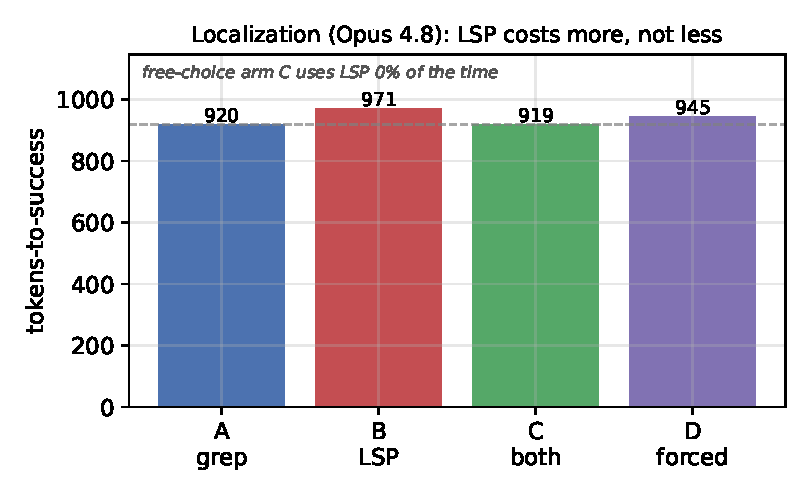
\includegraphics[width=0.62\textwidth]{figs/fig1_localization.pdf}
\caption{\textbf{Localization (Opus 4.8): the LSP costs more, not less.} Tokens-to-success by arm. The
LSP-only arm (B) is $6\%$ more expensive than grep-only (A) at identical $100\%$ success. The
free-choice arm (C) collapses onto grep (it uses the LSP $0\%$ of the time), and forcing semantic-first
(D) \emph{reduces} success to $89\%$. On localization where the issue text names the symbol, semantic
retrieval is a token tax.}
\end{figure}

On localization where the issue text typically \emph{names} the symbol, \textbf{semantic retrieval costs
more tokens, not fewer}. Decisively, in arm C the agent used the LSP \textbf{zero times} --- C collapses
onto A. Forcing semantic-first (D) \emph{reduced} success and the agent still resisted (4 semantic vs.\
51 grep calls). This confirms \textbf{Prediction 2}, \emph{refutes} the localization half of
\textbf{Prediction 1} (for symbol-named localization, semantic retrieval is a tax), and confirms
\textbf{Prediction 3} emphatically: the habit gap is so strong that forcing backfires.

\subsection{Model sweep --- LSP helps weak models, taxes strong ones}

Same localization tasks, three models, 72 episodes each.

\begin{center}\small
\begin{tabular}{@{}lrrcr@{}}
\toprule
Model & grep T2S & lsp T2S & lsp vs.\ grep & free-choice semantic use \\
\midrule
Opus 4.8 & 920 & 971 & \textbf{$+6\%$} & 0\% \\
Sonnet 4.6 & 606 & 1{,}319 & \textbf{$+118\%$} & 4\% \\
Haiku 4.5 & 11{,}911 & 8{,}799 & \textbf{$-26\%$} & 6\% \\
\bottomrule
\end{tabular}
\end{center}

\begin{figure}[h]
\centering
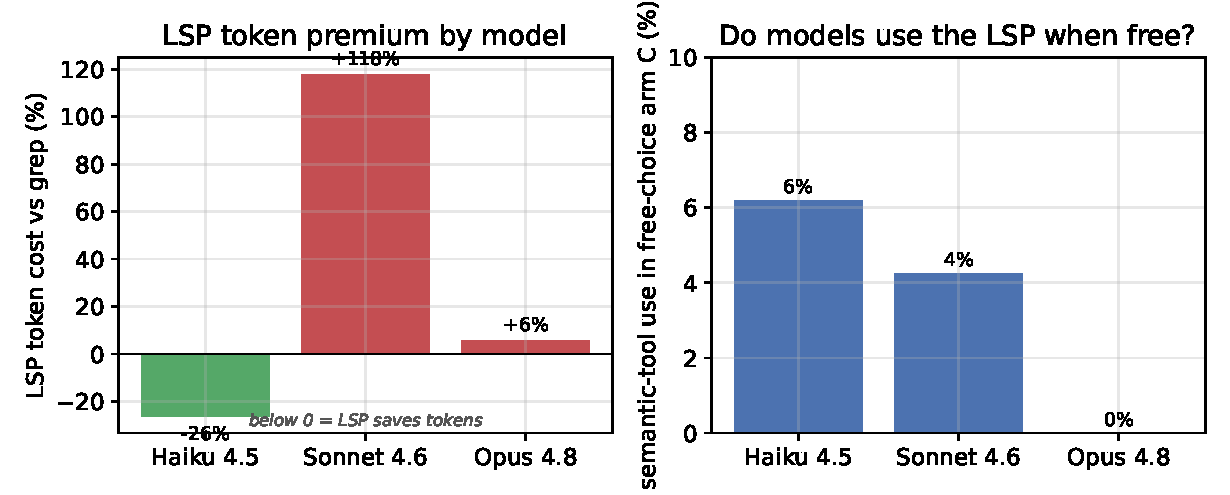
\includegraphics[width=0.92\textwidth]{figs/fig2_models.pdf}
\caption{\textbf{Capability dependence and the universal grep habit.} \emph{Left:} the LSP token premium
over grep, by model. Only the weakest model (Haiku) \emph{saves} tokens with the LSP ($-26\%$); both
capable models pay a premium (Opus $+6\%$, Sonnet $+118\%$). \emph{Right:} how often each model uses a
semantic tool in the free-choice arm C. Every model defaults to grep --- even Haiku, which would save
$26\%$, uses the LSP only $6\%$ of the time. Giving the tool is not enough.}
\end{figure}

The \textbf{capability dependence} is the headline: the weakest model (Haiku --- which flails with grep
noise, ${\sim}12$k tokens and 13+ turns per task) is the \emph{only} one that \textbf{saves} tokens with
the LSP; both capable models pay a premium. Semantic retrieval is a crutch for weak models and a tax for
strong ones. And the grep preference is \textbf{universal}: free-choice semantic use is $0\%/4\%/6\%$.

\subsection{Reference-completeness --- LSP buys precision, not tokens, and cannot fix recall}

Task = list \emph{every} call site of a target function, scored by F1 against \code{pyright}'s reference
set. (We switched the oracle from \code{pylsp} to \code{pyright} after finding jedi's reference
resolution too incomplete to serve as ground truth --- itself a finding about LSP quality variance.)
Five cross-file \code{requests} functions $\times$ 4 arms $\times$ 3 rollouts, Opus~4.8.

\begin{center}\small
\begin{tabular}{@{}lrrrr@{}}
\toprule
Arm & mean F1 & precision & recall & tokens \\
\midrule
A grep-only & 0.706 & 0.76 & 0.67 & 1136 \\
B lsp-only & \textbf{0.778} & \textbf{1.00} & 0.66 & 1347 ($+19\%$) \\
C grep+lsp (free) & 0.706 & 0.76 & 0.67 & 1354 \\
D forced-semantic & 0.710 & 0.77 & 0.67 & 1499 \\
\bottomrule
\end{tabular}
\end{center}

\begin{figure}[h]
\centering
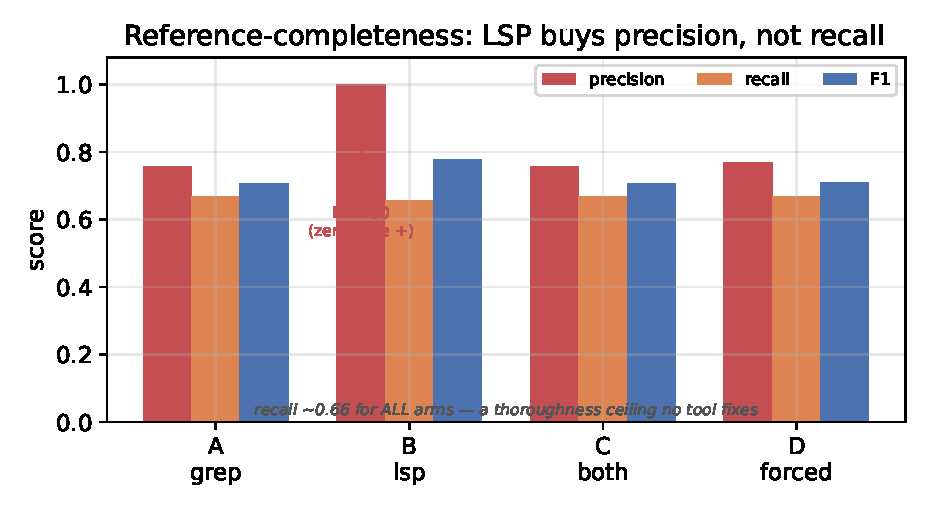
\includegraphics[width=0.72\textwidth]{figs/fig3_reference.pdf}
\caption{\textbf{Reference-completeness: the LSP buys precision, not recall.} Precision, recall, and F1
by arm. The LSP arm (B) achieves \emph{perfect precision} (1.00 --- zero false call sites) versus grep's
0.76, and wins on F1. But \textbf{recall is identical ($\sim$0.66) across all arms}: no tool helps the
agent find \emph{more} true call sites. The missing third is an agent-thoroughness ceiling, not a
retrieval problem.}
\end{figure}

Here --- on \code{find\_references}' home turf --- \textbf{the LSP wins on accuracy} (F1 $0.778$ vs.\
$0.706$), the \emph{opposite} of localization: the task class decides whether semantic retrieval helps.
The decomposition is the real result. The entire gain is \textbf{precision}: B reports zero false call
sites (1.00) vs.\ grep's 0.76 ($\sim$24\% of grep hits are false positives --- comments, strings,
unrelated same-named symbols). \textbf{Recall is identical ($\sim$0.66) across all four arms}: neither
tool helps the agent find \emph{more} true sites --- the missing third is an \emph{agent-thoroughness}
problem, not a retrieval one, which the LSP cannot fix. The precision gain costs $\sim$19\% more tokens,
appears on every cross-file target ($+0.06$ to $+0.13$ F1), and vanishes on the one single-file target
(both arms F1 $=1.00$). Free-choice arm C reverts to grep's profile --- the agent forgoes the precision
gain even where it exists.

\begin{figure}[h]
\centering
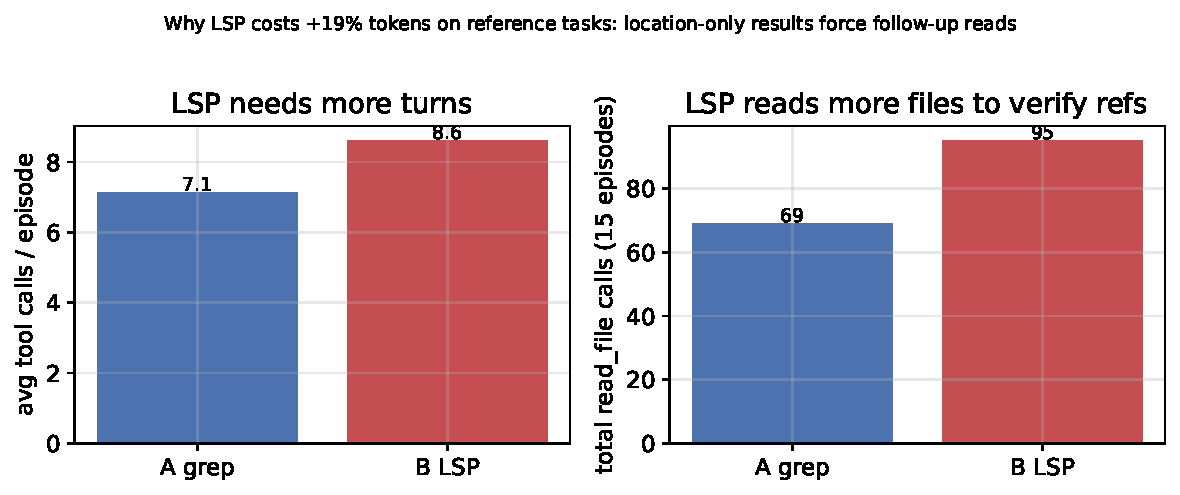
\includegraphics[width=0.92\textwidth]{figs/fig4_why.pdf}
\caption{\textbf{Why the LSP costs $+19\%$ tokens on reference tasks.} Per-tool-call token cost is nearly
identical between arms ($163$ vs.\ $160$); the difference is \emph{call/turn count}. \emph{Left:} the LSP
arm issues more tool calls per episode. \emph{Right:} it issues far more \code{read\_file} calls.
\code{find\_references} returns \emph{locations only} (\code{path:line}), so the agent must open those
files to verify each call site; \code{grep} returns the matching line's \emph{content inline}, often
needing no follow-up read. Each extra turn re-bills the accumulated conversation context --- so the cost
compounds. An LSP tool that returned the referenced line inline would likely erase the penalty while
keeping precision~$=1.00$ (an actionable H-interface fix).}
\end{figure}

\subsection{Synthesis}

Across two task classes and three models, a single conditional structure holds:

\begin{quote}
\textbf{``Does an LSP save tokens?'' --- in general, no.} On symbol-named \emph{localization} it
\emph{costs} tokens (a tax that grows with model strength). On \emph{reference-completeness} it does not
save tokens either; it buys \emph{precision} at a $\sim$19\% premium and cannot fix the recall
bottleneck. It saves tokens only for the \emph{weakest} model, as a crutch against lexical noise. And
across every condition, \textbf{agents default to \code{grep} when free --- forgoing the LSP even where
it helps.}
\end{quote}

This argues against ``LSP-always'' and for \textbf{(a)} an adaptive router keyed on task class, model
capability, and lexical-noise level, and \textbf{(b)} training the \emph{when-to-go-semantic} competence
into the policy --- because handing the model the tool is empirically insufficient.

\section{Limitations and threats to validity}\label{sec:limits}

The \S\ref{sec:results} results are a \textbf{pilot}: \textbf{(i)~single repository, small N} ---
\code{requests}, a small library the models likely saw in pretraining; 6 localization tasks and 5
reference targets, 3 rollouts each. Directions are robust; effect sizes (e.g.\ Sonnet's $+118\%$) are
pilot-scale and will move with more data. \textbf{(ii)~Oracle quality} drove a mid-study change from
\code{pylsp} to \code{pyright} (jedi was too incomplete to be ground truth) --- itself a finding, and a
caution that any single LSP-as-truth inherits that server's blind spots. \textbf{(iii)~Task coverage}
--- we did not run the \emph{edit} tasks end-to-end with test execution, arm E (static repo-map), or
large repositories where per-symbol LSP cost and the static-index trade-off would bite.
\textbf{(iv)~Language/server} --- Python with \code{pylsp}/\code{pyright}; the originally-motivating
\textbf{TypeScript} case (statically typed, most reliable references) is untested and is the most
important next stratum. \textbf{(v)~Harness specificity} and \textbf{(vi)~token accounting} (we count
total context tokens; caching can change billed cost). \textbf{(vii)~Provenance} as in \S2.

\section{Conclusion}

``Does an LSP save tokens'' is not a tooling opinion --- it is a measurable statement about retrieval
precision under a token budget, and it has gone unmeasured in public while being near-universally
asserted. We reduced it to a single metric (\emph{tokens-to-success at iso-accuracy}), a five-arm
ablation, and a mapping of three failure modes onto movable variables --- and ran a pilot that turns the
prior into first numbers. The pilot answer is \textbf{conditional, and in the common case negative}: on
symbol-named localization the LSP \emph{costs} tokens (a tax growing with model strength); on
reference-completeness it buys \emph{precision}, not token savings, at a $\sim$19\% premium and cannot
lift the recall ceiling; it nets a saving only for the weakest model. Underneath sits the most robust
finding: \textbf{every model defaults to \code{grep} when the LSP is merely available.} That is why the
durable solution is not ``add an LSP'' but to make the routing --- and eventually the semantic competence
itself --- \textbf{native to the policy rather than a brittle external layer}, the direction
RL-from-language-server-feedback already points. The contribution is to replace an assertion with a
measurement, and a blanket recommendation with a conditional one. The honest next step is scale: more
repositories, the edit and static-index arms, and the TypeScript stratum.

\appendix
\section{Source provenance}
\textbf{Fetch-verified (F):} \url{https://github.com/oraios/serena};
\url{https://github.com/isaacphi/mcp-language-server}; \url{https://aider.chat/docs/repomap.html};
arXiv:2604.18413, 2510.22907, 2606.11864, 2605.18747 (full abstracts). \\
\textbf{Established background (K), not fetched:} SWE-bench (Jimenez et al., 2023); SWE-agent ACI (Yang
et al., 2024); AutoCodeRover; Moatless.

\end{document}
